\documentclass[a4paper,10pt]{article}

% packages
\usepackage[utf8]{inputenc} % allows usage of spanish special characters
\usepackage[spanish,english]{babel} % english dictionary for proper hyphenation
\usepackage{amsmath} % math expressions
\usepackage{upgreek} % upright greek letters for math
\usepackage{txfonts} % nice fonts 
\usepackage{authblk} % author affiliations
\usepackage{graphicx} % images
\usepackage{float} % image positioning
\usepackage{multirow} % allows merging cells in tables
\usepackage{makecell} % more table customization
\usepackage{mathtools} % nice matrices
\usepackage{units} % nice fractions
\usepackage{rotating} % rotated text
\usepackage{caption} % customization of figure/table captions
\usepackage{subcaption} % collages of multiple images
\usepackage{hyperref} % hyperlinks
\usepackage{nameref} % cross-references between draft and supplementary material
\usepackage{zref-xr,zref-user} % more cross-references formatting
\zxrsetup{toltxlabel}
\zexternaldocument*{supp}
\usepackage[square,numbers,sort&compress]{natbib}
\usepackage[table,xcdraw]{xcolor} % text and table background colors
\usepackage[margin=2.5cm]{geometry} % margins
\usepackage{lineno} % line numbers
\usepackage{textcomp} % special characters (some references break if this isn't loaded?)
\usepackage{mdframed} % to easily handle boxes
\usepackage[misc]{ifsym} % use \Letter symbol for corresponding author

% customization
\setcounter{Maxaffil}{0} % affiliations
\renewcommand\Affilfont{\itshape\small} % style of affiliations text
\makeatletter\renewcommand{\@biblabel}[1]{#1.}\makeatother % change [number] for number. in reference list
\addto{\captionsenglish}{\renewcommand{\bibname}{References}}
\newcommand{\idea}[1]{\textcolor{red}{#1}}
\newcommand{\mr}{\textcolor{red}{\textbf{[missing ref(s)]}}}
\newcommand{\Burl}[1]{\url{#1}}
\zxrsetup{toltxlabel} % cross references: draft & suppl mat
\zexternaldocument*[M-]{draft}
\hypersetup{
  colorlinks = true,
  citecolor=  black,
  linkcolor = {blue},
  filecolor = cyan % controls color of external ref, if used
}
\captionsetup[figure]{font=small, labelfont={bf}, labelformat={default},
   labelsep=period, name={Figure}} % custom figure captions
\captionsetup[table]{font=small, labelfont={bf}, labelformat={default},
   labelsep=period, name={Table}} % custom table captions
\hypersetup{citecolor={blue}}
\definecolor{lightgray}{gray}{0.9}
\newcommand{\figref}[2][]{%
  \hyperref[{#2}]{%
    Figure~\ref*{#2}%
    \ifx\\#1\\%
    \else
      #1%
    \fi
  }%
}
\newcommand{\tableref}[1]{%
  \hyperref[{#1}]{%
   Table~\ref*{#1}%
  }%
}
\newcommand{\methodsref}[1]{%
  \hyperref[{methods:#1}]{%
   Methods:~\nameref*{methods:#1}%
  }%
}

% title, authors, affiliations
\title{Top-down versus bottom-up cohesiveness in microbial community coalescence}
\author[1 *]{Juan Diaz-Colunga}
\author[1 *]{Nanxi Lu}
\author[1,2 *]{Alicia Sanchez-Gorostiaga}
\author[1]{Chang-Yu Chang}
\author[1]{Helen S. Cai}
\author[3]{Joshua E. Goldford}
\author[4]{Mikhail Tikhonov}
\author[1 \Letter]{Álvaro Sánchez}
\affil[1]{Department of Ecology \& Evolutionary Biology
and
Microbial Sciences Institute,
Yale University, New Haven, CT, USA}
\affil[2]{Department of Microbial Biotechnology,
Centro Nacional de Biotecnología (CNB-CSIC), Cantoblanco, Madrid, Spain}
\affil[3]{Physics of Living Systems, Department of Physics,
Massachusetts Institute of Technology, Cambridge, MA, USA}
\affil[4]{Department of Physics,
Center for Science \& Engineering of Living Systems,
Washington University in St. Louis, St. Louis, MO, USA}

\affil[$\textrm{\Letter}$]{\normalfont~alvaro.sanchez@yale.edu}
\affil[*]{\normalfont~These authors contributed equally}
\date{}



  
\begin{document}

\linenumbers

\maketitle

\begin{abstract}
  
The abstract goes here.
  
\end{abstract}

\section*{Introduction}\label{intro}

Microbial communities often invade one another.
This has been observed, for instance, 
in river courses where terrestrial microbes mix with aquatic microorganisms
\cite{Mansour2018,Luo2020,Vass2021}
or in soil communities being invaded as a result of
tillage and outplanting \cite{Rillig2016} or by
aerially dispersed bacteria and funghi \cite{Evans2019}.
Gut microbiomes can invade external communities
through the host animal secretions \cite{Dutton2021},
and the skin microbiota is also subject to
invasions when making contact with environmental sources of microbes \cite{Vandegrift2019}.

The phenomenon by which entire microbiomes invade one another has been termed
\textit{community coalescence} \cite{Rillig2015}.
Ecologists have long contemplated the idea that interactions between multiple co-invading species
can produce correlated invasional outcomes
\cite{Gilpin1994,Simberloff1999,Grosholz2005,Simberloff2006,Gurevitch2006,Green2011,
Livingston2013,Prior2015,Rillig2015,OLoughlin2017,Castledine2020}.
However, and
in spite of its clear potential importance, the role of coalescence in microbiome assembly is
only beginning to be addressed and little is known about the mechanisms that govern it and its
potential implications.
Early mathematical models of community-community invasions \cite{Gilpin1994,Toquenaga1997}
as well as more recent work
\cite{Tikhonov2016,Tikhonov2017,Vila2019,Lechon2021}
suggest that high-order invasion effects are common
during community coalescence. Communities that have a previous history of coexistence may exhibit an
emergent ``cohesiveness'' which produces correlated invasional outcomes among species from the
same community \cite{Livingston2013,Sierocinski2017}.
The situation where ecological partners in the invading community recruit each other into the final
coalesced community has been called \textit{ecological co-selection} \cite{Rillig2017,Sierocinski2017}.

The mechanisms of ecological co-selection during community coalescence are still poorly understood.
Do a few key species recruit everyone else, or are collective interactions among all species
(including the rarer members of the community) relevant for coalescence outcomes?
While it is reasonable to expect species with larger population sizes to have a proportionally oversized effect,
natural communities tend to be highly diverse \cite{Louca2016}
and
the role played by the less abundant species has long been subject to debate \cite{Winfree2015}.
Laboratory cultures have also been found to contain uneven distributions of multiple strains that feed
off the metabolic secretions of the dominant species \cite{Rosenzweig1994,Goldford2018}.
The fate of these sub-dominant taxa may be dependent on the invasional success of their dominant
species, or, alternatively, the dominant itself may owe its dominance (at least in part) to cross-feeding
or other forms of facilitation from the rarer members of the population.
These scenarios would give rise to ``top-down'' or ``bottom-up'' community cohesiveness, respectively.
Either of these forms of co-selection could, in principle, be positive (recruitment) or negative (antagonism),
as illustrated in \figref[e]{fig1}.
Which of these situations are typically found in nature?
Previous theoretical and computational studies suggest that the answer is determined by the type and
strength of the interactions of the community members with one another and with the environment
\cite{Tikhonov2016,Vila2019,Lechon2021},
but addressing this question has been experimentally challenging in the past \cite{Rillig2017,Sierocinski2017}.

In previous work, we have shown that a large amount of soil and plant microbiomes can be cultured
\textit{ex situ} in synthetic minimal environments with a single supplied limiting resource under serial
growth-dilution cycles \cite{Goldford2018} (\figref[a-b]{fig1}). Under these conditions, environmental
microbiomes spontaneously re-assemble into complex multi-species communities sustained by dense
cross-feeding facilitation networks \cite{Goldford2018}. In addition,
and just like in natural consortia,
species abundance distributions
in these communities are generally long-tailed and uneven (\figref[d]{fig1} and \figref{figS1}),
with the dominant (most abundant) species typically comprising most of the biomass ($\text{median}=46\%$,
\figref{figS1}). Because these communities are easy to manipulate and grow in high throughput, and
are largely made up by culturable members, they represent good test cases to investigate ecological
co-selection during community coalescence. Here we focus on the dominants and ask whether they can
co-select or be co-selected by the sub-dominant species in their communities (henceforth referred to as
their \textit{cohorts}, \figref[c]{fig1}).

Our results indicate that co-selection varies in direction and strength depending on the supplied limiting
resource.
This primary resource, in turn, has been shown to
shape the structure and interactions of the communities \cite{Estrela2020}.
We observe that, when top-down co-selection is weak, bottom-up co-selection can be very strong,
with positive co-selection being far more common than negative co-selection.
\iffalse
Our results confirm that positive top-down co-selection is common, but its effects are weak.
In contrast, bottom-up co-selection can be very strong, and positive co-selection is far more common
than negative co-selection.
\fi
We then turn to a Microbial Consumer-Resource Model (MicroCRM)
\cite{Goldford2018,Marsland2019,Marsland2020}
that is able to capture the dynamics of microbial communities dominated by metabolic interactions,
as is the case for the ones assembled in our experimental conditions \cite{Goldford2018,Estrela2020}.
We show that the empirically observed trends in ecological co-selection are reproduced
with minimal model assumptions, and that the recurrence of top-down and bottom-up co-selection
is determined by the configuration of the cross-feeding networks in the MicroCRM.
Our findings indicate that collective interactions play an important role at dictating community structure
during coalescence.

\section*{Results \& Discussion}\label{results-discussion}

We collected eight natural microbiomes from different soil and plant environmental samples
(\figref[a]{fig1})
and used them to inoculate our synthetic communities, which were stabilized 
in serial batch-culture biorreactors for 84 generations in synthetic minimal media containing either
glutamine or citrate as the only supplied carbon source
(\figref[b]{fig1}, \methodsref{community-assembly}).
We chose these two carbon sources because they are metabolized through different
pathways in bacteria \cite{Dimroth2004,Forchhammer2007},
and we hypothesize that communities assembled in either resource will be supported by
cross-feeding networks of distinct sets of metabolites \cite{Goldford2018,Estrela2020}
thus leading to potentially variable degrees of community cohesiveness
and coalescence outcomes \cite{Tikhonov2016,Tikhonov2017,Castledine2020,Lechon2021}.
We isolated the dominant species of every community
(\methodsref{dominants})
and identified them by Sanger-sequencing their 16S rRNA gene
(\methodsref{sequencing}), which correctly matched the dominant
Exact Sequence Variant (ESV) \cite{Callahan2016,Callahan2017} found through
community-level 16S Illumina sequencing
(\figref{figS1}).
These dominants remained at high frequency after seven additional transfers
with the exception of two of the citrate communities and one of the glutamine
communities (where the dominants were presumably a transiently dominating species)
that were excluded from further analysis
(\figref{figS1}).
Similarly, pairs of communities where the dominants shared a same 16S sequence
and had similar colony morphology were excluded
(\figref{figS1}).

\subsubsection*{Top-down ecological co-selection}

If communities being coalesced were highly cohesive from the top-down,
the dominant species would co-select the rarer members of its community during coalescence
(\figref[e]{fig1}, left panels).
In this scenario, we would expect the outcome of community coalescence to be predicted by
which of the two dominants is most competitive in pairwise competition.
Analogously, competition between dominants should be affected only weakly by the presence or
absence of the cohorts, that would play a passive role under these conditions.
To test this hypothesis, we performed all pairwise competitions between dominant species
in glutamine and citrate environments by mixing them 1:1 on their native media and propagating
the cultures for seven serial transfers, roughly 42 generations
(\methodsref{competitions}).
We then carried out all possible pairwise community coalescence experiments by mixing
equal volumes of the communities and propagating the resulting cultures for seven extra
transfers
(\figref[f]{fig1}).
\iffalse
and we quantified coalescence outcomes using the similarity between the coalesced and the
invasive communities
(\methodsref{metrics}).
\fi
The frequencies of all species in both community-community and dominant-dominant competitions
were determined by 16S Illumina sequencing
(\methodsref{sequencing}).

We found that, for communities assembled in the glutamine environment,
the relative frequency of a dominant against another in head-to-head pairwise competition
is barely predictive of its relative frequency against that same other dominant when the
cohorts are present too, i.e. during community coalescence
(\figref[a]{fig2} red dots, $R^2=0.04$, $p>0.05$).
This correlation is significantly higher for the citrate communities
 (\figref[a]{fig2} blue dots, $R^2=0.83$, $p<10^{-8}$).
This suggests that, in the glutamine environments, head-to-head competition of dominants
is heavily influenced by higher order effects introduced by the rare taxa of the communities.
On the other hand, the cohorts seem to play a more passive role in the citrate environments.
To test the effects of top-down co-selection at the community level,
we quantified the distances between the invasive and coalesced communities
using the relative Bray-Curtis similarity (\methodsref{metrics})
and compared them to the outcomes of the pairwise competitions between dominants alone.
We again noticed differences between glutamine and citrate communities:
for the former,
the pairwise competitive ability of an invasive dominant
is only weakly predictive of the performance of the invasive community in coalescence
(\figref[b]{fig2} left panel, $R^2=0.15$, $p<0.05$).
For the latter,
the structure of the coalesced communities tends to be more strongly dictated by the
result of the dominant-dominant competition
(\figref[b]{fig2} middle panel, $R^2=0.57$, $p<10^{-4}$).
Alternative quantifications of community distance yield similar results,
with weaker effects when the metric used
accounts only for the presence/absence of specific species and not for their relative abundance in
the communities
(\figref{figS2}).
All these metrics include the presence of the dominant species themselves. To better disentangle the effect
that these dominants have on the other members of their communities, we repeated the analysis this time
excluding the dominant species from the compositional data, finding that our results still hold
(\figref{figS3}).

Together, these observations suggest that the strength of top-down co-selection depends on
the environment where communities are assembled and coalescence takes place.
Communities stabilized with citrate as the primary supplied resource
display a strong degree of top-down cohesiveness,
with the fates of the sub-dominant species determined to a large extent by dominant-dominant
pairwise competition. This competition is, in turn, only weakly affected by the presence of the cohorts.
For glutamine communities, although some level of top-down co-selection is consistent with our data,
the cohorts do not appear to just be passively responding to their dominants
but rather playing an active role in community coalescence.

To investigate the determinants of top-down co-selection and the factors modulating its strength,
we ran a set of simulations of community coalescence. We used a Microbial Consumer-Resource
Model (MicroCRM) \cite{Goldford2018,Marsland2019} as implemented in the Community Simulator package
for Python \cite{Marsland2020}
(\hyperref[box1]{Box~1}).
We chose this modeling framework because
communities assembled under our experimental conditions (natural microbiomes re-assembled into
multispecies communities through serial growth-dilution cycles in synthetic minimal media
with a single carbon source)
have been shown to be sustained by dense metabolic cross-feeding networks
\cite{Goldford2018,Estrela2020}
for which the MicroCRM provides a good description.
Based on previous experimental work
\cite{Harcombe2014,Pinu2018,Estrela2020},
we allowed different species in our model
to secrete different sets of byproducts when metabolizing a same resource
(\hyperref[box1]{Box~1}).
\iffalse
this choice is discussed in \hyperref[box1]{Box~1}.
\fi
To reproduce our experimental protocol \textit{in silico},
we first generated a library of resources and two non-overlapping pools of species.
Each pool was used to seed a collection of 100 invasive
and 100 resident communities respectively
by randomly choosing 50 species and
allowing them to stabilize through 20 growth-dilution cycles.
We then mixed these stable communities in pairs to simulate our coalescence
and dominant-dominant competition experiments
(\methodsref{sim}).
We found that the MicroCRM was able to capture a correlation between
the head-to-head pairwise competition of dominants
and the outcome of community coalescence
(\figref[b]{fig2}, right panel),
further supporting the idea that top-down ecological co-selection can consistently
emerge from metabolic interactions across species.

\iffalse
[Maybe this ``outro'' sentence is not even necessary]
Our experiments had shown that this correlation varied
across communities assembled in the glutamine and citrate environments
(\figref[b]{fig2}, left and middle panels),
which led us to investigate the determinants of the strength and direction
of ecological co-selection in our model.

\fi
\clearpage

\begin{mdframed}
\internallinenumbers
\subsubsection*{Box 1: A Microbial Consumer-Resource Model for community coalescence}
\label{box1}

The Microbial Consumer-Resource Model (MicroCRM) \cite{Goldford2018,Marsland2019,Marsland2020}
is a modeling framework based on the classic MacArthur's consumer resource model
\cite{MacArthur1970}.
It encodes the dynamics of a system with $S$ species and $M$ resources
in terms of a consumer preference matrix $\mathbf{c}$ and a metabolic matrix $\mathbf{D}$,
with an additional set of parameters controlling
the species maintenance costs ($m_i$ for species $i$),
the resource energy densities ($w_\alpha$ for resource $\alpha$),
the energy to growth rate conversion factor ($g_i$ for species $i$)
and the leakage fraction, i.e. the amount of energy lost as byproducts when a resource is consumed
($l_\alpha$ for resource $\alpha$).
The element $c_{i\alpha}$ of the consumer preference matrix
represents the uptake rate of resource $\alpha$ by
species $i$ (although the relationship between $c_{i\alpha}$ and the uptake rate can be more
complex in modeling scenarios that are not considered here,
see \cite{Goldford2018,Marsland2019,Marsland2020}).
Experimental evidence suggests that individual species can secrete different sets of metabolites
to the environment when growing on a same primary resource
\cite{Harcombe2014,Pinu2018,Estrela2020}.
Thus, we define $\mathbf{D}$ as a three-dimensional matrix
where the element $D_{i\beta\alpha}$ represents the energy flux in the form of resource $\beta$
that is secreted by species $i$ when it metabolizes resource $\alpha$.
Note that $D_{i\beta\alpha}$ need not be equal to $D_{j\beta\alpha}$ if $i \neq j$
(see illustration below).
\iffalse
For our simulations,
the elements of $\mathbf{c}$ are sampled from a gamma distibution,
while the elements of $\mathbf{D}$ are sampled from a Dirichlet distribution
to ensure that the normalization condition $\sum_\beta D_{i\beta\alpha} = 1$
is satisfied for every $i$ and $\alpha$.
\fi
\iffalse
The sampling is performed so that species belonging to a same family
tend to secrete more similar byproducts when consuming a same resource
(see \methodsref{sim} and \cite{Marsland2019,Marsland2020}),
as supported by experimental observations
\cite{Harcombe2014,Pinu2018,Estrela2020}.
\fi

\bigskip
\begin{center}
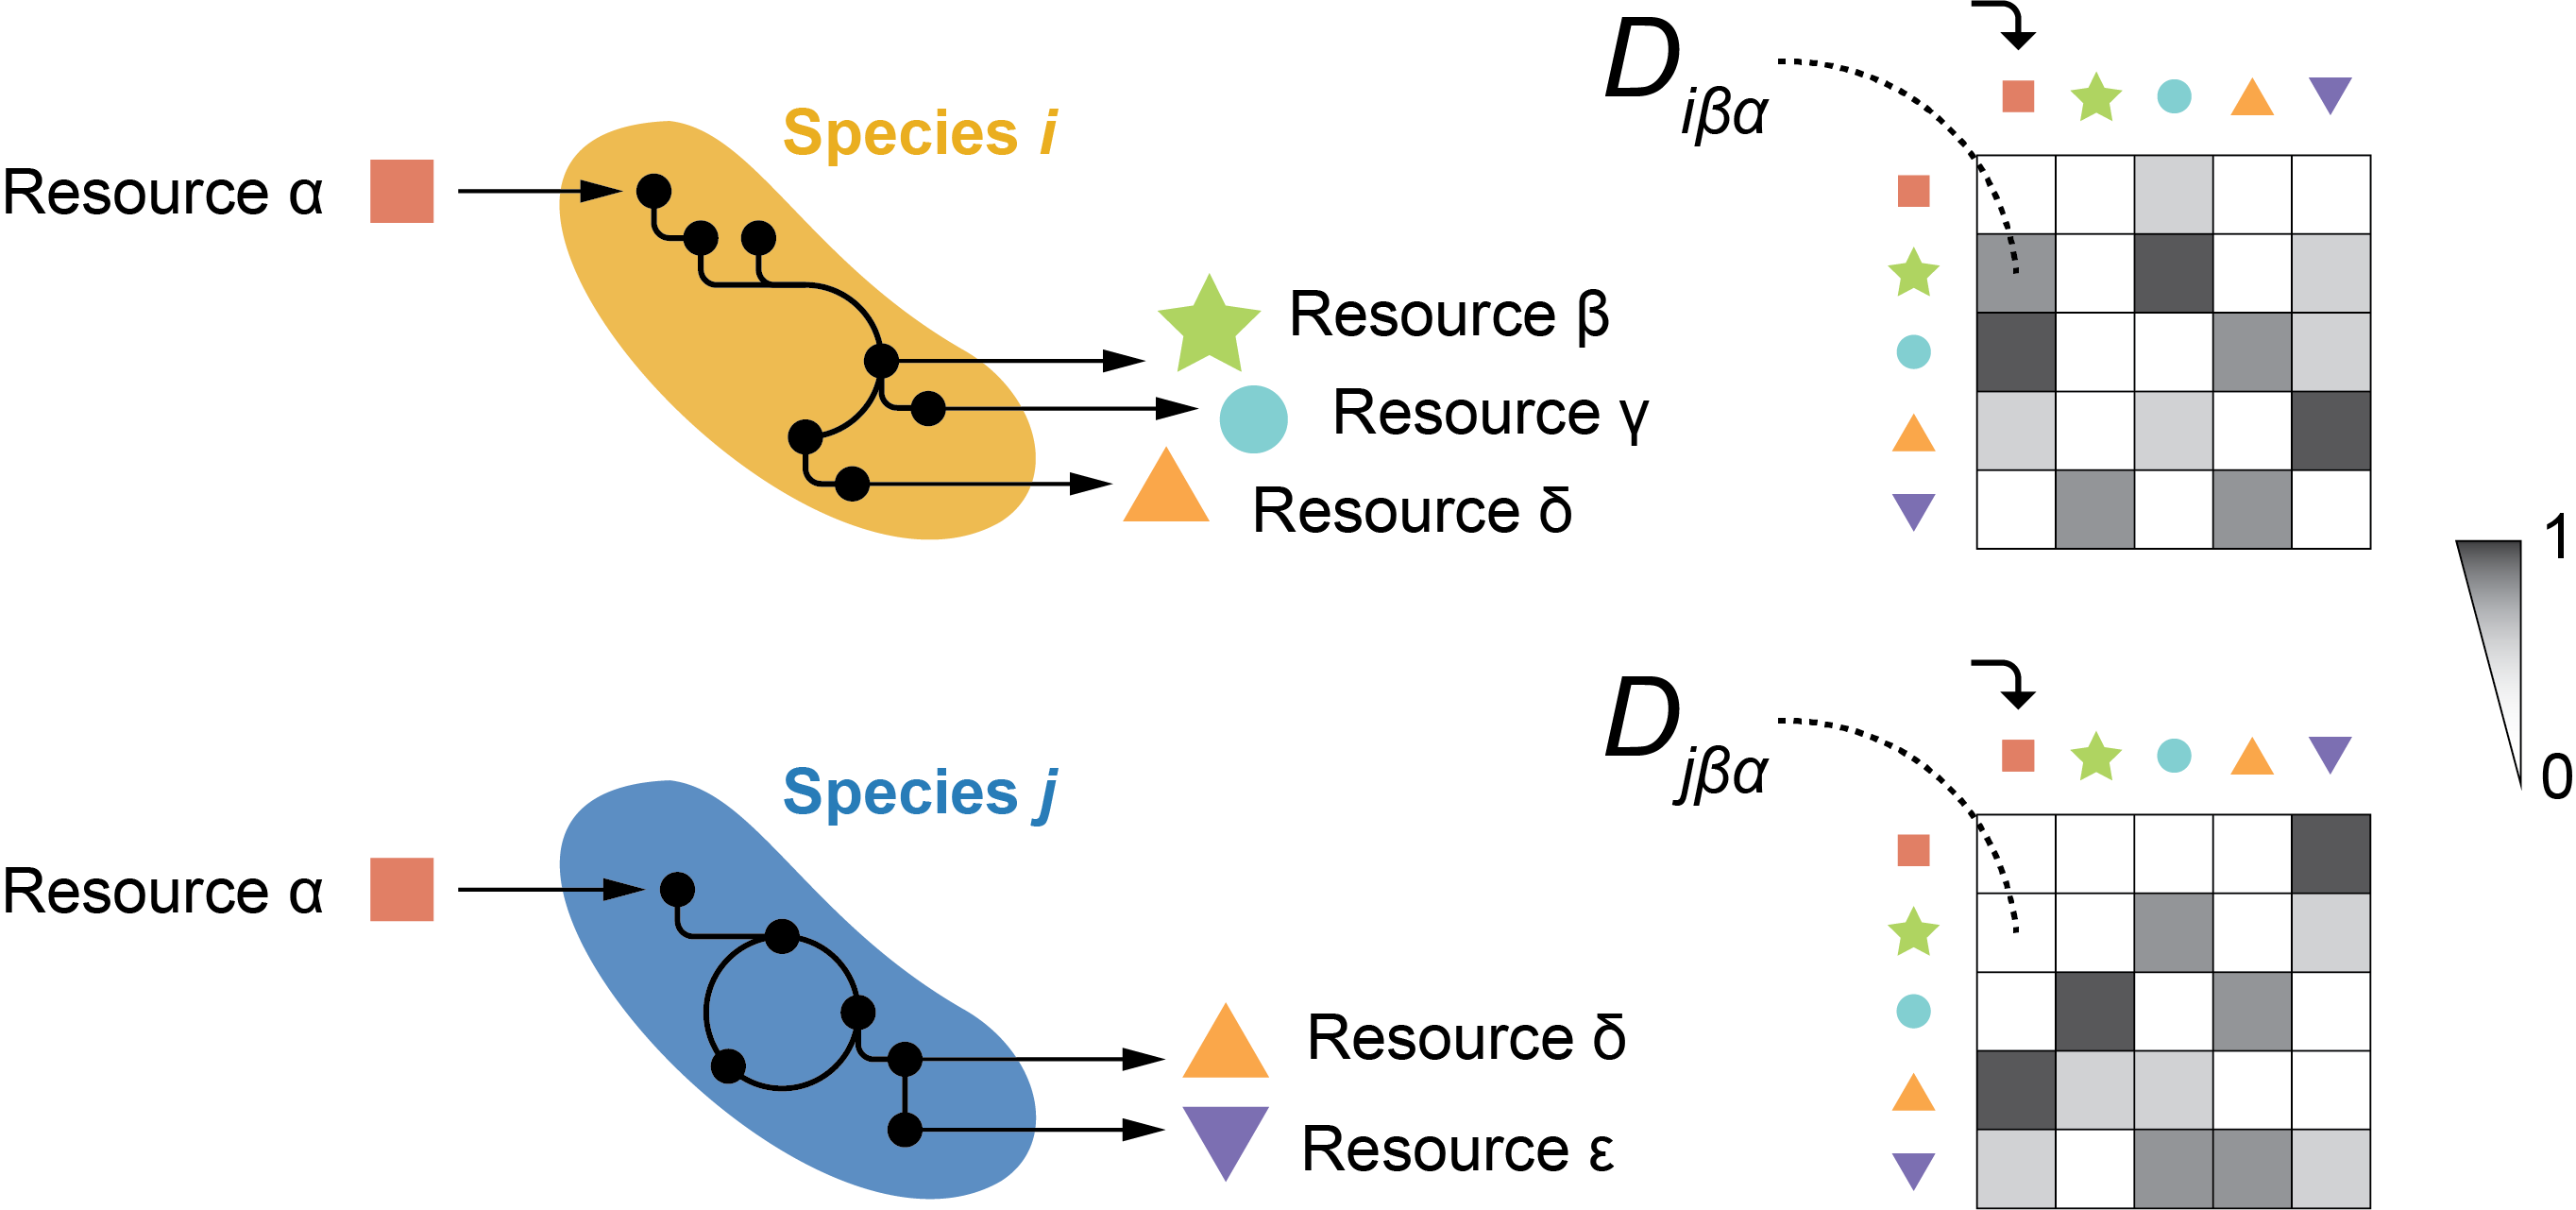
\includegraphics[width=11cm,keepaspectratio]{figs/figBox_v3.png}
\end{center}
\bigskip

The following equations describe the kinetics of the abundances
of the $i$-th species (denoted as $N_i$)
and the $\alpha$-th resource (denoted as $R_\alpha$):

\begin{equation}
\frac{dN_i}{dt} = 
g_i N_i
\left[
\sum_\alpha \left( 1-l_\alpha \right)
w_\alpha c_{i\alpha} R_\alpha
- m_i
\right]
\label{eq:crm-n}
\end{equation}

\begin{equation}
\frac{dR_\alpha}{dt} = 
- \sum_j N_j c_{j\alpha} R_\alpha
+ \sum_j \sum_\beta N_j c_{j\beta} R_\beta
\left[
l_\beta D_{j\alpha\beta} \frac{w_\beta}{w_\alpha}
\right]
\label{eq:crm-r}
\end{equation}
%
These equations can take slightly different forms in certain cases,
e.g. if the primary resource is supplied continuously instead of at the beggining
of each growth cycle \cite{Marsland2019,Marsland2020},
but they are a good approximation for the community dynamics between consecutive
serial dilutions in our setup.
Here, we assembled \textit{in silico} communities by randomly
sampling a set of species from a pool,
then integrating equations \ref{eq:crm-n} and \ref{eq:crm-r},
diluting the final abundances,
replenishing the primary resource (by default denoted as $R_0$),
and repeating the process until generational equilibrium was achieved
(\methodsref{sim}).
Coalescence simulations were carried out following the same logic,
this time seeding the coalesced communities by mixing the invasive and resident
communities instead of sampling from a species pool.

\bigskip
\end{mdframed}

\clearpage

\iffalse
We found that, for communities assembled in the glutamine environment,
the pairwise competitive ability of an invasive dominant
is only weakly predictive of the performance of the invasive community in coalescence
(as quantified by the relative Bray-Curtis similarity between the coalesced and invasive communities),
but this correlation was stronger for the citrate communities
(\figref[a]{fig2}, $R^2=0.15$, $p<0.05$ for glutamine and $R^2=0.57$, $p<10^{-4}$ for citrate).
Alternative quantifications of community distance yielded similar results,
with weaker effects when the metric used
accounted only for the presence/absence of specific species and not for their relative abundance in
the communities
(\figref{figS2}).
All these metrics include the presence of the dominant species themselves. To better disentangle the effect
that these dominants have on the other members of their communities, we repeated the analysis this time
excluding the dominant species from the compositional data, finding that our results still hold
(\figref{figS3}).
Furthermore, we observed that, in the glutamine communities,
the relative frequency of a dominant against another in head-to-head pairwise competition
is barely predictive of its relative frequency against that same other dominant when the
cohorts are present too, i.e. after coalescence
(\figref[a]{fig2} red dots, $R^2=0.04$, $p>0.05$).
On the other hand, pairwise competition between dominants of the citrate communities
is highly correlated with the relative abundance of said dominants in community coalescence
 (\figref[a]{fig2} blue dots, $R^2=0.83$, $p<10^{-8}$).

Together, these results suggest that the strength of top-down co-selection depends on
the primary resource supplied to the coalesced communities.
Communities assembled with citrate as the primary supplied resource
display a strong degree of top-down co-selection,
with the fates of the sub-dominant species determined to a large extent by dominant-dominant
pairwise competition. This competition is, in turn, only weakly affected by the presence of the cohorts.
For glutamine communities, although some level of top-down co-selection is consistent with our data,
the cohorts do not appear to be passively responding to their dominants.
Instead, evidence suggests that the cohorts might be playing an active role in community coalescence.
This finding led us to investigate the potential role of bottom-up ecological co-selection
(\figref[e]{fig1}, right panels), i.e. whether in some cases the dominants may be co-selected
for or against by their cohorts.
\fi

\subsubsection*{Bottom-up co-selection during community coalescence}

Our data indicates that the primary resource supplied to the communities can modulate
the effect that the cohorts have in the dominants pairwise competition
(\figref[a]{fig2})
and the strength of top-down co-selection
(\figref[b]{fig2}, left and middle panels).
The fact that
our model captures these trends
suggests that this might be a result of the metabolic interactions
between community members, including the rarer taxa.
To investigate the potential role of the cohorts in coalescence,
 i.e. whether the dominants may be co-selected for or against by them
(\figref[e]{fig1}, right panels),
we ran a new set of simulations
this time invading resident communities with the dominants alone
(\methodsref{sim}).
We compared the invasion success of the dominants in isolation with respect to our previous
simulations where they invaded accompanied by their cohorts.
The invasion success of the dominants was quantified by their relative abundance
in the final stabilized communities.
Whenever positive bottom-up ecological co-selection is strong, we expect to see dominants
reaching higher invasion success with their cohorts than by themselves
(\figref[b]{fig3}, green shaded region).
On the other hand, a high degree of bottom-up antagonism would result in dominants
invading more effectively alone than in the presence of their cohorts
(\figref[b]{fig3}, red shaded region).
Alternatively, if both forms of bottom-up co-selection are weak, we would see a similar invasion success
regardless of the presence or absence of the cohort
(\figref[b]{fig3}, gray shaded region).

\figref[b]{fig3} shows that, in the simulations,
many dominants could not invade on their own
(or could only do so at very low final relative abundances, below 0.1)
but were able to reach high frequencies when they were accompanied by their cohorts.
This indicates that positive bottom-up co-selection is frequent and potentially very strong,
while negative bottom-up co-selection is far more uncommon.
We then asked whether the ability of the pairwise competition of dominants
to predict coalescence outcomes was dependent on the strength of bottom-up co-selection.
We divided our simulations into two subsets:
the first one was comprised of the instances where positive bottom-up co-selection was strong
(i.e. dots in the green shaded region of \figref[b]{fig3}),
the second set included all other cases
(dots near the diagonal of \figref[b]{fig3}).
We reexamined our original simulations and plotted the frequency of the invasive dominant
in pairwise competition with the resident dominant versus the relative similarity between
the invasive and coalesced communities,
i.e. the same plot as in \figref[b]{fig2}, for each subset.
We found that when bottom-up positive co-selection is strong,
the pairwise competition of dominants is not predictive of coalescence outcomes
(\figref[c]{fig3}, left panel) and vice-versa (\figref[c]{fig3}, right panel).

We then asked whether this trend was also observed \textit{in vitro}.
We went back to our laboratory cultures
and carried out a new round of experiments where we invaded the resident communities
with the invasive dominants alone
(\methodsref{competitions}).
After stabilization, we quantified species abundance through 16S Illumina sequencing
(\methodsref{sequencing}).
Again, we observed that bottom-up co-selection is far more common in its
positive than in its negative form
(\figref[d]{fig3}).
Interestingly, bottom-up recruitment appears to be more frequent in the glutamine
environments than in the citrate ones,
consistent with our hypothesis that metabolic interactions among species
are key in determining the strength and direction of ecological co-selection.
We then repeated our analysis in \figref[c]{fig3},
this time splitting our data according to the observed strength of bottom-up
co-selection instead of the primary carbon source
as we had done in \figref[b]{fig2}.
Our findings were in line with the model prediction:
pairwise competition between dominants is only predictive of coalescence outcomes
if bottom-up co-selection is weak
(\figref[e]{fig3}, $R^2=0.07$, $p>0.05$ when bottom-up co-selection is strong;
$R^2=0.37$, $p<10^{-4}$ when bottom-up co-selection is weak).

\iffalse
To test which of these situations was more common in our conditions,
we performed a new round of invasion experiments where each dominant invaded every
other community in isolation (\methodsref{competitions}). The dominant-invaded
communities were then propagated for seven serial transfers, and the final
community compositions were determined by 16S Illumina sequencing.
We compared the relative abundances reached by the dominants in these experiments
with the relative abundances of the same dominants in community coalescence
(i.e. when they invade with their cohorts).
\figref[b]{fig2} shows that, for communities assembled in citrate environments,
the cohorts had little effect and the dominants were able to invade with comparable
success regardless of being accompanied by them.
This was expected since we had seen that coalescence between citrate communities
tended to be determined by top-down co-selection.
However, glutamine communities displayed a different behavior.
A large number of dominants (roughly 50\%) that were not able to invade by themselves
(or could only do so at very low final relative abundances, below 0.1)
were able to reach much higher frequencies when they invaded together with their cohorts,
which indicates that positive bottom-up co-selection is common in our experiments.
In contrast, negative co-selection appears to be rare and no instances of it were
observed in our experiments.
\fi

\iffalse
\subsubsection*{Simulations of community coalescence with a Consumer-Resource Model}

To better understand the mechanisms of ecological co-selection in our experiments,
we ran a set of simulations of community coalescence. We used a Microbial Consumer-Resource
Model (MicroCRM) \cite{Goldford2018,Marsland2019} implemented in the Community Simulator package
for Python \cite{Marsland2020}. We chose this modeling framework because
communities assembled under our experimental conditions (natural microbiomes re-assembled into
multispecies communities through serial growth-dilution cycles in synthetic minimal media
with a single carbon source)
have been shown to be
sustained by dense metabolic cross-feeding networks
\cite{Goldford2018,Estrela2020},
for which the MicroCRM provides a good description.
We implemented a new feature in the package that makes individual species
able to secrete different sets of byproducts when consuming a same resource
(\methodsref{sim}).
We also used sparse metabolic matrices, equivalent to assuming that species secrete only a few
types of byproducts when consuming a resource. These assumptions are supported by the experimental
observation that individual species can indeed secrete different sets of few metabolites
to the environment when consuming a primary resource
\cite{Harcombe2014,Pinu2018}. \mr cite Sylvie here?
We reason that these choices are necessary to potentially generate community cohesiveness:
if the secretions of all species were roughly similar, the effect of interchanging members of
a community would be minimal. But in practice, species with a history of coexistence make up
cohesive communities with highly specific cross-feeding structures \cite{Goldford2018,Estrela2020}.
In short,
we reproduced our experimental protocol \textit{in silico}
by generating a library of species that we divided into two pools. Each pool was used to seed a
collection of invasive and resident communities, that were allowed to stabilize through 20
growth-dilution cycles. We then mixed pairs of these stable communities to carry out our coalescence
and dominant-dominant competition experiments,
as well as the invasion experiments from the dominants alone.
A full description of our modeling framework can be found in the \methodsref{sim} section.

We carried out two sets of simulations under two different regimes.
In one case, we generated a library of 30 resources divided into 3 resource classes
(\methodsref{sim}). This corresponds to a situation where the digestion of a resource
can yield a wide variety of secreted byproducts.
We refer to this scenario as the \textit{complex resource} regime.
Our second set of simulations was performed under a \textit{simple resource} regime, where we
generated a library of only 15 resources belonging to a same class.
For the simple resource, we found that coalescence outcomes were highly correlated with
the competitive ability of the community dominants in pairwise competition
(\figref[c]{fig2}),
indicating a large degree of top-down positive co-selection.
These dominants were able to reach similar fractions in the final communities when invading alone
with respect to when invading with their cohorts
(\figref[d]{fig2}),
suggesting that bottom-up co-selection is weak in this scenario.
On the other hand,
simulations under the complex resource regime evidenced weak top-down co-selection but 
common and strong bottom-up recruitment (\figref[e-f]{fig2}), with negative co-selection remaining rare.
Simulations suggest that community cohesiveness is dependent on the metabolic interactions among species,
which is in line with previous findings \cite{Goldford2018, Estrela2020}.
These interactions are determined by the metabolic profile of the primary resource in the conditions
of our simulations and, in turn, modulate the strength and direction of ecological co-selection.
\fi

\subsubsection*{Understanding the mechanisms of ecological co-selection: a minimal model of community coalescence}

To better understand the underlying mechanisms that govern
the emergence of ecological co-selection,
we developed a minimal model of community coalescence.
This model is comprised of two communities with two species each
as illustrated in \figref[a]{fig4}.
Within each community, the dominant species
($\mathrm{s}_1$ and $\mathrm{s}_3$ in the resident and invasive communities
respectively)
is able to utilize the primary resource that is supplied externally ($\mathrm{R}_1$).
As a result of $\mathrm{R}_1$ metabolism,
the dominants secrete a single byproduct off which
the sub-dominant species ($\mathrm{s}_2$ and $\mathrm{s}_4$ respectively) can feed.
Finally, these sub-dominants secrete an additional resource that can again
be metabolized by the respective dominants.
This is the simplest structure where both top-dwn and bottom-up
cohesiveness can emerge, with their relative strengths being determined
by how effectively the species can utilize each other's metabolic byproducts.
Several parameters can modulate the direction of community cohesiveness,
and even in this simple model there can be complex interactions between them.
For instance, a sub-dominant that is very efficient at metabolizing the dominant
secretions will therefore be a strong producer of secondary secretions,
in turn increasing the metabolic flow towards the dominant itself.

\subsubsection*{Community hierarchy regulates the strength of bottom-up co-selction}

How do the ideas above scale to more complex and diverse communities?

We reason that the choice of species-specific metabolic architectures is necessary to potentially generate
cohesiveness at the community level during coalescence.
If the secretions of all species were identical (or only slightly different),
higher order cross-feeding effects would be very unspecific:
the establishment of new invasive species
--given that they could outcompete resident taxa within their metabolic niches,
i.e. more effectively feed off the same resource or set of resources as them--
would not alter (or only do so moderately)
the metabolic flows through the rest of the community's cross-feeding network.
On the other hand, said network could undergo a profound and further-reaching restructuring
if the invasive species secreted very different sets of metabolites with respect to the resident ones,
potentially disabling existing niches and/or enabling new ones
where more invaders could be co-selected.
For a similar reason, we argue that the sparsity of the metabolic matrix could also modulate
the emergence of cohesiveness in the face of coalescence.
A dense metabolic matrix corresponds to a situation where all species secrete a wide
variety of byproducts.
New-coming invasive species that secrete similar byproducts as resident ones
--even if they do so in different relative amounts--
might only induce moderate quantitative changes in the metabolic fluxes.
But if the sets of secretions are qualitatively different, co-selection of species adapted to
each of those sets becomes possible.
These ideas are supported by experimental observations
suggesting that species with a history of coexistence make up
cohesive communities with highly specific cross-feeding configurations
\cite{Rosenzweig1994,Goldford2018,Estrela2020}.

\subsubsection*{Conclusions}

\iffalse
Ideas for the conclusions: results and previous theoretical and experimental work on different systems (and on the
general relationship between metabolic interactions and community structure) suggest that...
the strength and direction of ecological co-selection is determined by the underlying metabolic networks that
shape the structure and interactions of communities assembled in synthetic minimal environments
during coalescence.
These networks are modulated by the supplied primary resource in our conditions.
When top-down co-selection is weak, bottom-up positive co-selection can be very strong, while negative
co-selection remains rare in our experiments.
ALSO: we have only discussed metabolic interactions here. Other forms of facilitation are possible
(and probably more relevant in specific natural settings)... but cohesiveness FOR SURE arises from metabolic interactions
in our experiments, and we know the effect is ultimately metabolic because the MicroCRM captures it
(actually both forms of it, top-down and bottom-up).
\fi

Understanding the mechanisms underlying the responses of microbial communities to invasions is
an essential but poorly understood question in microbial ecology \cite{Rillig2015}.
Theory has suggested that communities may exhibit an emergent cohesiveness
\cite{Gilpin1994,Livingston2013,Tikhonov2016,Tikhonov2017},
leading to members of the same community recruiting one another during
community-community invasions.
Our results provide direct experimental evidence of ecological co-selection in a large number
of community coalescence experiments,
and highlight the critical role played by the rarer, sub-dominant species in the generation
of community cohesiveness.

Our data suggests that the strength and direction of ecological co-selection is modulated
by the underlying metabolic networks that shape the structure of
communities assembled in synthetic minimal conditions
\cite{Goldford2018,Estrela2020}.
This network is in turn regulated by the supplied primary carbon source
in our minimal laboratory conditions.
This idea is supported by the observation that a Microbial Consumer-Resource Model
captures the trends observed experimentally when we enable a large variation
in the metabolic fluxes across species.
The model also predicts a trade-off between the strength of bottom-up co-selection
and the ability of dominant-dominant pairwise competition to dictate coalescence outcomes,
which we have confirmed experimentally.
These observations,
together with previous results in different systems \cite{Sierocinski2017} as well as
theoretical predictions
\cite{Gilpin1994,Toquenaga1997,Tikhonov2016,Tikhonov2017,Vila2019,Lechon2021},
suggest that collective interactions between microbes
and the environment should be generically expected to produce ecological co-selection
during community coalescence.

Additional work will be necessary to further clarify the relationship between
metabolic feedbacks, community cohesiveness and ecological co-selection.
The experimental system that we introduced in this work can be easily expanded so that
large numbers of community coalescence experiments can be carried out in parallel.
It thus represents a promising tool to explore the properties of microbial community
coalescence in high throughput
and test quantitative theories about its role in microbiome assembly.
On the other hand, coalescence of communities under different settings
(e.g. in spatially structured environments)
might be governed by additional factors.
Understanding them and quantifying their relative contributions in natural communities
remains an open question in ecology.

\clearpage











\section*{Methods}\label{methods}

\subsubsection*{Stabilization of environmental communities in simple synthetic environments}
\label{methods:community-assembly}

Communities were stabilized \textit{ex situ} as described in \cite{Goldford2018}.
In short, environmental samples (soil, leaves...) within one meter radius in eight different
geographical locations were collected with sterile
tweezers or spatulas into 50mL sterile tubes (\figref[a]{fig1}).
One gram of each sample was allowed to
sit at room temperature in 10mL of phosphate buffered saline (1$\times$PBS) containing
200$\upmu$g/mL cycloheximide to suppress eukaryotic growth.
After 48h, samples were mixed 1:1 with 80\% glycerol and kept frozen at $-80^\circ$C.
Starting microbial communities were prepared by scrapping the frozen stocks into
$200\upmu$L of 1$\times$PBS and adding a volume of $4\upmu$L to $500\upmu$L
of synthetic minimal media (1$\times$M9) supplemented with $200\upmu$g/mL cycloheximide
and 0.07 C-mol/L glutamine or sodium citrate as the carbon source in 96 deep-well plates
(1.2mL; VWR).
Cultures were then incubated still at $30^\circ$C to allow for re-growth.
After 48h, samples were fully homogenized and biomass increase was followed by measuring
the optical density (620nm) of $100\upmu$L of the cultures in a Multiskan FC plate reader
(Thermo Scientific).
Communities were stabilized \cite{Goldford2018} by passaging $4\upmu$L of the cultures into
$500\upmu$L of fresh media (1$\times$M9 with the carbon source)  every 48h for a total of
12 transfers at a dilution factor of 1:100,
roughly equivalent to 80 generations per culture (\figref[b]{fig1}).
Cycloheximide was not added to the media after the first two transfers.

\subsubsection*{Isolation of dominant species}\label{methods:dominants}

For each community, the most abundant colony morphotype at the end of the ninth transfer
was selected (\figref[c]{fig1}),
resuspended in $100\upmu$L 1$\times$PBS and serially diluted (1:10).
Next, $20\upmu$L of the cells diluted to $10^{-6}$ were plated in the corresponding synthetic
minimal media and allowed to regrow at $30^\circ$C for 48h. Dominants were then identified,
inoculated into $500\upmu$L of fresh media and incubated still at $30^\circ$C for 48h.
After this period, the communities stabilized for eleven transfers and the isolated dominants
were ready for the competition experiments at the onset of the twelfth transfer.

\subsubsection*{Coalescence, competition and invasion experiments}
\label{methods:competitions}

All possible pairwise dominant-dominant and community-community
competition experiments
were performed by mixing equal volumes ($4\upmu$L) of each of the eight
communities or eight dominants at the onset of the twelfth transfer.
Competitions were set up in their native media,
i.e. in $500\upmu$L of 1$\times$M9 supplemented with 0.07 C-mol/L of
either glutamine or citrate in 96 deep-well plates.
Plates were incubated at $30^\circ$C for 48h.
Pairwise competitions were further propagated for seven serial transfers
(roughly 42 generations, \figref[f]{fig1}) by transferring $8\upmu$L of
each culture to fresh media ($500\upmu$L).

\subsubsection*{Determination of community composition by 16S sequencing}
\label{methods:sequencing}

The sequencing protocol was identical to that described in \cite{Goldford2018}.
Community samples were collected by spinning down at 3500rpm for 25min
in a bench-top centrifuge at room temperature;
cell pellets were stored at $-80^\circ$C before processing.
To maximize Gram-positive bacteria cell wall lysis,
the cell pellets were re-suspended and incubated at $37^\circ$C for 30min
in enzymatic lysis buffer (20mM Tris-HCl, 2mM sodium EDTA, 1.2\% Triton X-100)
and 20mg/mL of lysozyme from chicken egg white (Sigma-Aldrich).
After cell lysis, the DNA extraction and purification was performed using the
DNeasy 96 protocol for animal tissues (Qiagen).
The clean DNA in $100\upmu$L elution buffer of 10mM Tris-HCl, 0.5mM EDTA
at pH 9.0 was quantified using Quan-iT PicoGreen dsDNA Assay Kit
(Molecular Probes, Inc.)
and normalized to 5ng/$\upmu$L in nuclease-free water (Qiagen)
for subsequent 16S rRNA Illumina sequencing.
16S rRNA amplicon library preparation was performed following a dual-index
paired-end approach \cite{Kozich2013}.
Briefly, PCR amplicon libraries of V4 regions of the 16S rRNA were prepared 
sing dual-index primers (F515/R805), then pooled and sequenced
using the Illumina MiSeq chemistry and platform.
Each sample went through a 30-cycle PCR in duplicate of $20\upmu$L
reaction volumes using 5ng of DNA each, dual index primers, and AccuPrime Pfx SuperMix (Invitrogen).
The thermocycling procedure includes a 2min initial denaturation step at
$95^\circ$C, and 30 cycles of the following PCR scheme:
(a) 20-second denaturation at $95^\circ$C,
(b) 15-second annealing at $55^\circ$C,
and (c) 5-minute extension at $72^\circ$C.
The duplicate PCR products of each sample were pooled, purified, and normalized
using SequalPrep PCR cleanup and normalization kit (Invitrogen).
Barcoded amplicon libraries were then pooled and sequenced using
Illumina Miseq v2 reagent kit, which generated 2$\times$250bp paired-end reads
at the Yale Center for Genome Analysis (YCGA).
The sequencing reads were demultiplexed on QIIME 1.9.0 \cite{Caporaso2010}.
The barcodes, indexes, and primers were removed from raw reads,
producing FASTQ files with both the forward and reverse reads for each sample,
ready for DADA2 analysis \cite{Callahan2017}.
DADA2 version 1.1.6 was used to infer unique biological exact sequence variants
(ESVs) for each sample
and na{\"i}ve Bayes was used to assign taxonomy using the SILVA version 123
database \cite{Wang2007,Quast2013}.

\subsubsection*{Metrics of community distance}
\label{methods:metrics}

Beta-diversity indexes between the invasive and coalesced communities
or the resident and coalesced communities were computed using various
similarity metrics. For two arbitrary communities with
ESV abundances represented by the vectors
$\mathbf{x} = \left( x_1, x_2, \cdots, x_S \right)$
and
$\mathbf{y} = \left( y_1, y_2, \cdots, y_S \right)$
(where $x_i$ and $y_i$ represent the relative abundance of the $i$th ESV in
each community respectively and $S$ is the total number of ESVs), the Bray-Curtis
similarity $BC \left( \mathbf{x}, \mathbf{y} \right)$ is calculated as
\cite{Bray1957}

\begin{equation}
BC \left( \mathbf{x}, \mathbf{y} \right) = 
\sum_i \mathrm{min} \left( x_i , y_i \right)
\label{eq:bray-curtis}
\end{equation}
%
The Jensen-Shannon similarity
$JS \left( \mathbf{x}, \mathbf{y} \right)$
is defined as one minus the Jensen-Shannon distance (which is, in turn,
the square root of the Jensen-Shannon divergence \cite{Lin1991})

\begin{equation}
JS \left( \mathbf{x}, \mathbf{y} \right) = 
1 - \sqrt{\frac{1}{2}KL \left( \mathbf{x}, \mathbf{m} \right) +
\frac{1}{2}KL \left( \mathbf{y}, \mathbf{m} \right)}
\label{eq:jensen-shannon}
\end{equation}
%
where $\mathbf{m} = \left( \mathbf{x} + \mathbf{y} \right)/2$ and KL denotes the
Kullback-Leibler divergence \cite{Kullback1951}

\begin{equation}
KL \left( \mathbf{x}, \mathbf{y} \right) = 
\sum_i x_i \; \mathrm{log_2} \left( \frac{x_i}{y_i} \right)
\label{eq:kullback-leibler}
\end{equation}
%
Using base-two logarithms ensures that the metric is bounded between 0 and 1.
The Jaccard similarity is given by
$J \left( \mathbf{x}, \mathbf{y} \right)$ \cite{Jaccard1912}

\begin{equation}
J \left( \mathbf{x}, \mathbf{y} \right) = 
\frac{\left|\; \mathbf{x} \cap \mathbf{y} \;\right|}
{\left|\; \mathbf{x} \cup \mathbf{y} \;\right|}
\label{eq:jaccard}
\end{equation}
%
Additionally, we quantified coalescence outcomes by examining the fraction of the endemic
cohort of the original communities that persists in the coalesced one. We call
$E \left( \mathbf{x}, \mathbf{y} \right)$ to the fraction of endemic species of
$\mathbf{x}$ that are also found in $\mathbf{y}$.

\iffalse

We denote this
metric as
$E \left( \mathbf{x}_\mathrm{I},
\mathbf{x}_\mathrm{R},
\mathbf{x}_\mathrm{C} \right)$.

\begin{equation}
E \left( \mathbf{x}_\mathrm{I},
\mathbf{x}_\mathrm{R},
\mathbf{x}_\mathrm{C} \right) = 
\left.
\sum_i
f \left( x_{\mathrm{I}i}, x_{\mathrm{R}i}, x_{\mathrm{C}i} \right)
\;
\middle/
\;
\sum_i
g \left( x_{\mathrm{I}i}, x_{\mathrm{R}i} \right)
\right.
\label{eq:endemic}
\end{equation}
%
where we have defined

\begin{equation}
\begin{split}
f \left( x_{\mathrm{I}i}, x_{\mathrm{R}i}, x_{\mathrm{C}i} \right) & =
\begin{cases}
    1 & \text{if } x_{\mathrm{I}i} > 0 \text{ and }
                   x_{\mathrm{R}i} = 0 \text{ and }
                   x_{\mathrm{C}i} > 0 \\
    0 & \text{otherwise}
\end{cases} \\
g \left( x_{\mathrm{I}i}, x_{\mathrm{R}i} \right) & =
\begin{cases}
    1 & \text{if } x_{\mathrm{I}i} > 0 \text{ and }
                   x_{\mathrm{R}i} = 0 \\
    0 & \text{otherwise}
\end{cases}
\end{split}
\label{eq:endemic-f}
\end{equation}

\fi

For all the metrics above, we quantified the relative similarity between the invasive
and the coalesced communities using relative metrics (denoted as $Q$):

\begin{equation}
Q \left( \mathbf{x}_\mathrm{I},
\mathbf{x}_\mathrm{R},
\mathbf{x}_\mathrm{C} \right) = 
\frac{F \left( \mathbf{x}_\mathrm{I},\mathbf{x}_\mathrm{C}\right)}
{F \left( \mathbf{x}_\mathrm{I},\mathbf{x}_\mathrm{C}\right)
+
F \left( \mathbf{x}_\mathrm{R},\mathbf{x}_\mathrm{C}\right)}
\label{eq:q}
\end{equation}
%
where the subindices I, R and C correspond to the invasive, resident and coalesced
communities respectively, and $F$ represents one of $BC$ (Bray-Curtis similarity), $JS$
(Jensen-Shannon similarity), $J$ (Jaccard similarity) or $E$ (endemic survival) defined above.

\subsubsection*{Simulations}\label{methods:sim}

We used the Community Simulator package \cite{Marsland2020} and included new
features for our simulations. In the package,
species are characterized by their resource uptake rates ($c_{i\alpha}$ for
species $i$ and resource $\alpha$), and they all
share a common metabolic matrix $\mathbf{D}$.
The element $D_{\alpha\beta}$
of this matrix represents the fraction of energy in the form of resource $\alpha$
secreted when resource $\beta$ is consumed.
Here we implemented a new operation mode
in which species can secrete different metabolites (and/or
in different abundances) when consuming a same resource.
We call $D_{i\alpha\beta}$ to the
fraction of energy in the form of resource $\alpha$ secreted \textit{by species
i} when consuming resource $\beta$.
In the Community Simulator underlying Microbial Consumer-Resource Model,
this means that the energy flux 
$J^{\mathrm{out}}_{i\beta}$ \cite{Goldford2018,Marsland2019}
now takes the form

\begin{equation}
J^{\mathrm{out}}_{i\beta} = \sum_\alpha D_{i\beta\alpha} l_\alpha J^{\mathrm{in}}_{i\alpha}
\label{eq:jout}
\end{equation}
%
The documentation for the Community Simulator contains detailed
descriptions of the model formulation,
parameters and package use.
For the updated package with
the new functionality, see \nameref{datacode}.

For our simulations,
we first generated a library of 2400 species divided into three specialist
families of 800 members each
and a generalist family of 240 members.
We split this library into two non-overlapping pools of 1320 species each.
We randomly sampled 50 species from each pool in equal ratios to seed
100 resident and
100 invasive communities respectively.
We then let grow and diluted the communities serially,
replenishing the primary
resource after each dilution.
We repeated the process 20 times to ensure generational equilibrium was
achieved \cite{Goldford2018}.
We then performed the \textit{in silico} experiments by using the
generationally stable communities to seed 100 coalesced communities
that were again stabilized as described previously.
Similarly, we identified the dominant (most
abundant) species of every resident and invasive community to carry out pairwise
competition and single invasion simulations.

Most other parameters were set to the defaults of the original Community Simulator
package, with the only exception of the maintenance costs ($m$) which are set to
zero for all species
(equivalent to assuming cell death is negligible through the duration of our growth cycles)
and the sparsity of the metabolic matrices ($s$) which is set to 0.9
to generate significant variability in the secretion fluxes across different species
(see main text).

\section*{Data \& code availability}\label{datacode}

Experimental data and code for the analysis, as well as code for the simulations
and the updated Community Simulator package with instructions for enabling the
new features are in \url{github.com/jdiazc9/coalescence}.

\section*{Acknowledgements}

The authors wish to thank Pankaj Mehta, Wenping Cui,
Robert Marsland and all members of the Sanchez laboratory
for many helpful discussions.
We also wish to express our gratitude to the Goodman laboratory at Yale
for technical help during the early stages of this project.
The funding for this work partly results from a Scialog Program
sponsored jointly by the Research Corporation for Science Advancement and
the Gordon and Betty Moore Foundation through grants to Yale University by the
Research Corporation and the Simons Foundation.








\clearpage

% references
\clearpage
\bibliographystyle{mystyle}
\bibliography{refs}








\clearpage

\section*{Figures}\label{figs}

\begin{figure}[!h]
\centering
\internallinenumbers
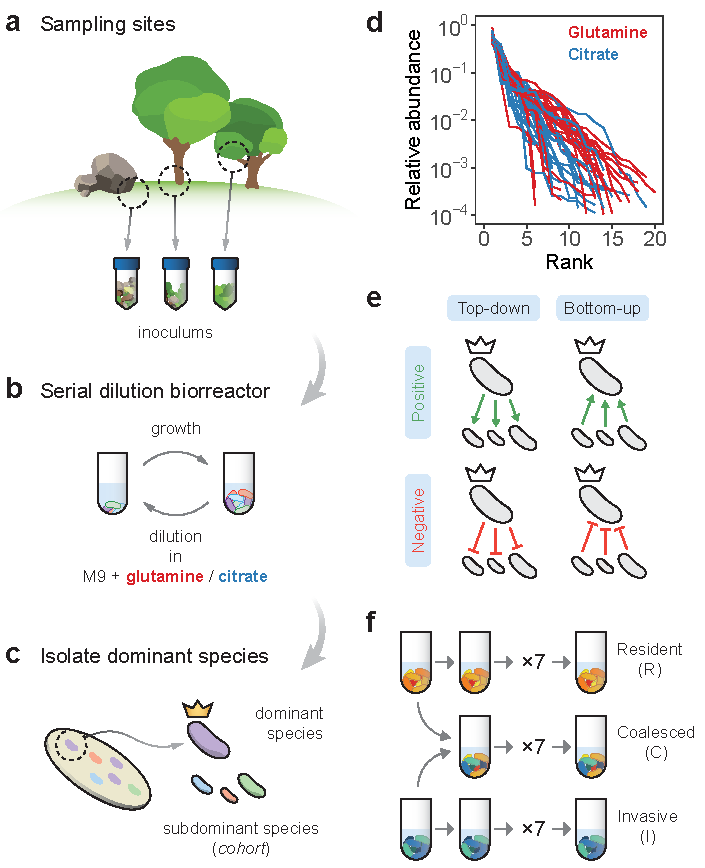
\includegraphics[scale=0.7,keepaspectratio]{figs/fig1.pdf}
\caption{\textbf{Overview of the experimental protocol.}
\textbf{a.}~Environmental samples collected from eight different locations were used
to inoculate our communities.
\textbf{b.}~Communities were stabilized in serial batch culture bioreactors
\cite{Goldford2018} in minimal synthetic media with glutamine or citrate as the
only supplied carbon source.
\textbf{c.}~Communities were plated in minimal media agar plates and the most abundant
species (the ``dominants") from each community were isolated. We refer to the set of
sub-dominant species as the ``cohorts".
\textbf{d.}~Rank-frequency distributions of all eight communities stabilized in either
glutamine (red) or citrate (blue), sequenced at a depth of $10^{-4}$ reads.
Three biological replicates per community are shown.
Community compositions are skewed and long-tailed.
\textbf{e.}~Our hypothesis is that ecological co-selection can take place from the top-down,
i.e. the dominant co-selecting the cohort, or from the bottom-up, i.e. the cohort co-selecting
the dominant. Both forms of co-selection can be positive (recruitment) or negative
(antagonism).
\textbf{f.}~Illustration of the protocol of our coalescence experiments. All pairs of
communities were inoculated into fresh minimal media supplemented with the same carbon
source where communities had been previously stabilized. The coalesced (C) and original
resident (R) and invasive (I) communities were then serially diluted and allowed to grow
for seven additional transfers.}
\label{fig1}
\end{figure}

\clearpage

\begin{figure}[!h]
\centering
\internallinenumbers
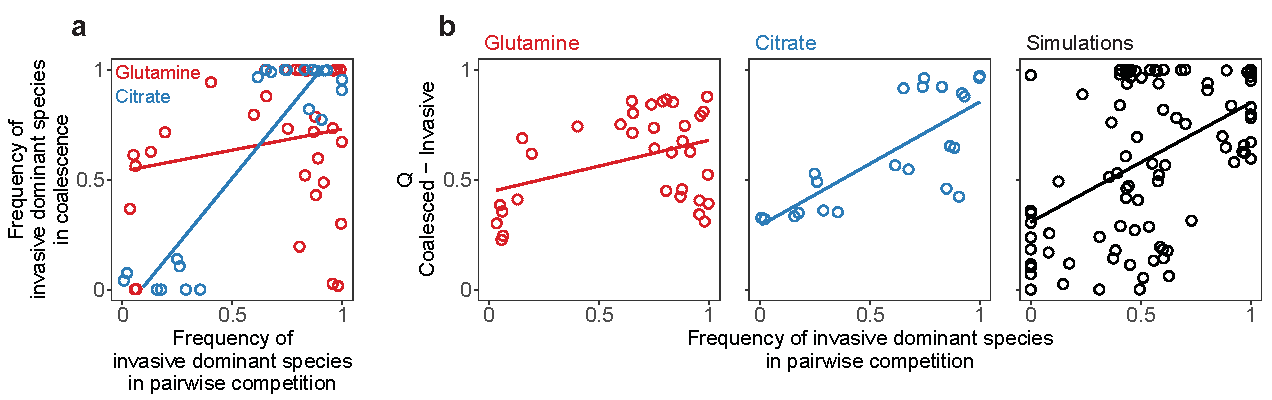
\includegraphics[scale=0.7,keepaspectratio]{figs/fig2_v3.pdf}
\caption{\textbf{Top-down co-selection in microbial community coalescence.}
\textbf{a.} Pairwise competition of dominants with or without their cohorts.
In the horizontal axis, we plot the frequency of the invasive dominant species
in head-to-head pairwise competition with the resident dominant.
In the vertical axis, we plot the same relative frequency when the two species compete
in the presence of their cohorts, i.e. during community coalescence.
$R^2=0.04$, $p>0.05$ for glutamine (red)
and $R^2=0.83$, $p<10^{-8}$ for citrate (blue).
\textbf{b.} Coalescence outcomes are quantified by the relative Bray-Curtis similarity
($Q$) between the coalesced and invasive communities.
These outcomes are predicted by the pairwise competition between the invasive and
resident dominant species.
Left panel (red): glutamine communities, $R^2=0.15$, $p<0.05$.
Middle panel (blue): citrate communities, $R^2=0.57$, $p<10^{-4}$.
A high correlation is consistent with a scenario of
strong top-down positive co-selection where dominants recruit their cohorts for the final
coalesced community. Two biological replicates per experiment are plotted individually.
Right panel (black): simulations with a Microbial Consumer-Resource Model are able
to capture these trends ($R^2=0.22$, $p<10^{-5}$).}
\label{fig2}
\end{figure}

\clearpage

\begin{figure}[!h]
\centering
\internallinenumbers
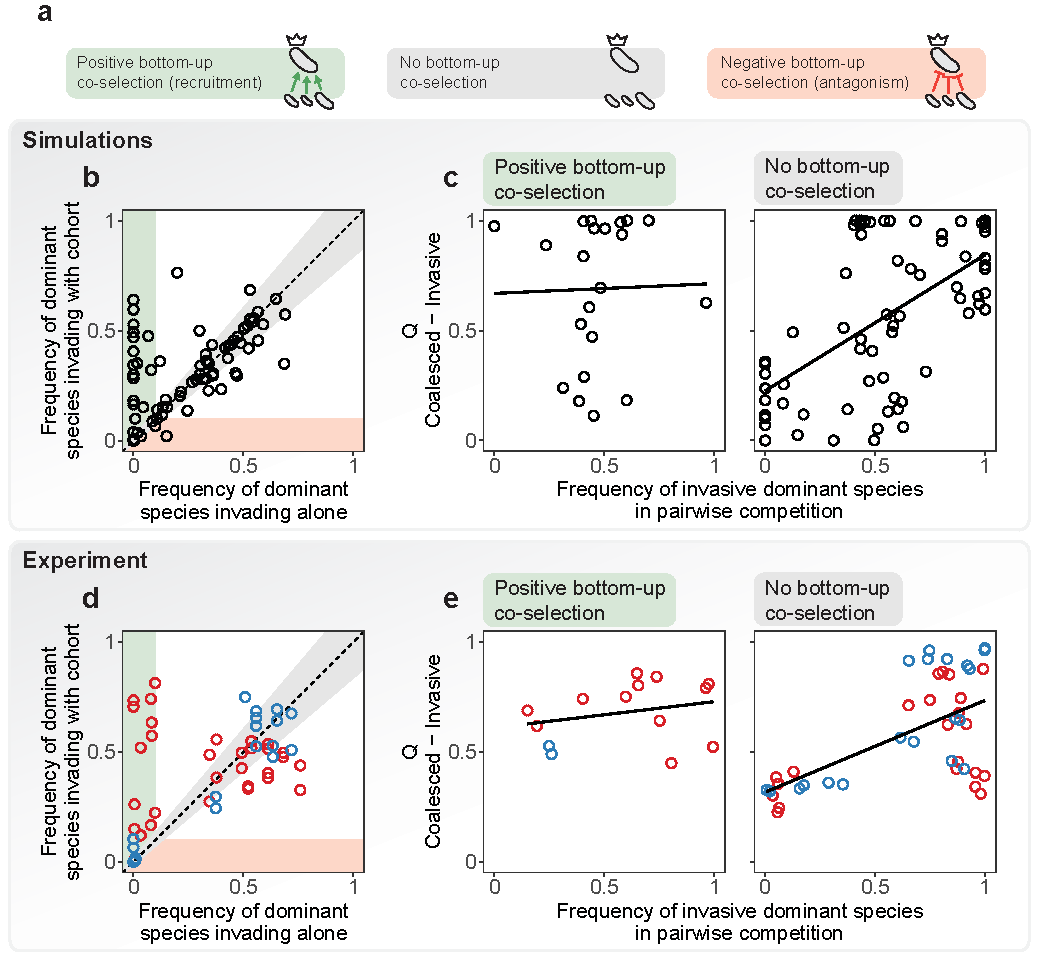
\includegraphics[scale=0.7,keepaspectratio]{figs/fig3.pdf}
\caption{\textbf{Trade offs between bottom-up and top-down ecological co-selection.}
\textbf{a.} We hypothesize that three scenarios are possible regarding bottom-up co-selection:
sub-dominant species could co-select for (green) or against (red) their dominant in coalescence,
or they could have no effect in the invasion success of the dominant taxa (gray).
\textbf{b.} Simulations with a Microbial Consumer-Resource Model suggest that positive bottom-up
co-selection is common and can be very strong, whereas negative bottom-up co-selection is rare.
We plot the frequency reached by the invasive dominants when invading the resident communities
in isolation versus the same frequency when invading together with their cohorts,
i.e. in community coalescence.
Points in the green/red area represent instances where the invasive dominant is able to invade
with higher/lower success when accompanied by its cohort, evidencing positive/negative
bottom-up co-selection.
Points around the diagonal (gray area) correspond to cases where the success of the invasive dominant
is only weakly affected by the presence or absence of its cohort.
\textbf{c.} We divided the data from our simulations into two sets according to whether
positive or no bottom-up co-selection was observed (that is, whether points fell into the green or gray
areas of panel b). Here we reproduce the plots in \figref[b]{fig2} for each set, representing the
result of the dominant head-to-head pairwise competition versus the outcome of community coalescence.
Left panel: when positive bottom-up co-selection is strong, head-to-head pairwise competition of dominants
is poorly predictive of coalescence outcomes
($R^2=0.00$, $p>0.05$).
Right panel: on the other hand, when bottom-up co-selection is weak coalescence outcomes are more
strongly dictated by the result of the dominant-dominant competition
($R^2=0.34$, $p<10^{-6}$).
\textbf{d.} Experiments show that in our conditions, positive bottom-up co-selection is indeed more
frequent and strong than negative bottom-up co-selection.
\textbf{e.} We reproduce the plots in panel c for our experimental data. This is equivalent to recreating
\figref[b]{fig2}, this time splitting our data by the strength of bottom-up co-selection
instead of by the carbon source provided to the communities.
Like simulations predicted, instances of community coalescence displaying strong positive bottom-up co-selection
yield a poor correspondence between dominant pairwise competition and coalescence outcomes
(left panel, $R^2=0.07$, $p>0.05$)
and vice-versa
(right panel, $R^2=0.37$, $p<10^{-4}$).}
\label{fig3}
\end{figure}

\clearpage

\begin{figure}[!h]
\centering
\internallinenumbers
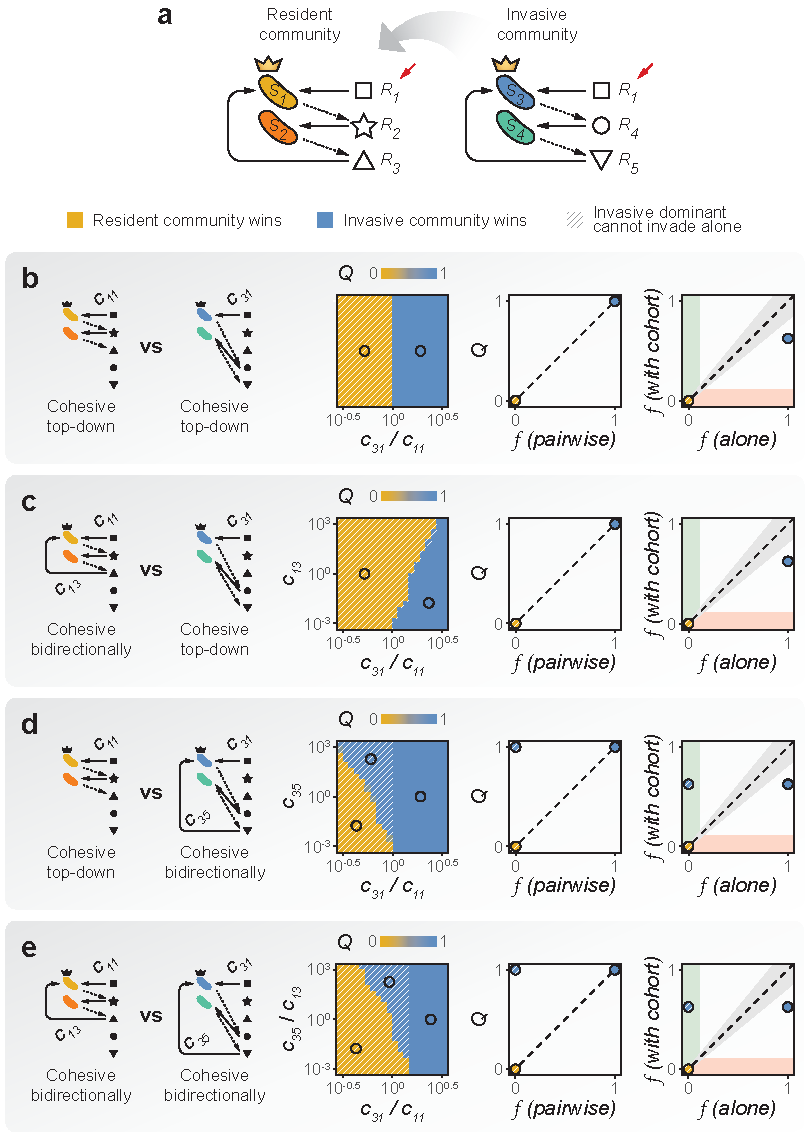
\includegraphics[scale=0.7,keepaspectratio]{figs/fig4_v2.pdf}
\caption{\textbf{A minimal model of community coalescence.}
\textbf{a.} Blablabla...
\textbf{b.} Blablabla...}
\label{fig4}
\end{figure}

\clearpage

\begin{figure}[!h]
\centering
\internallinenumbers
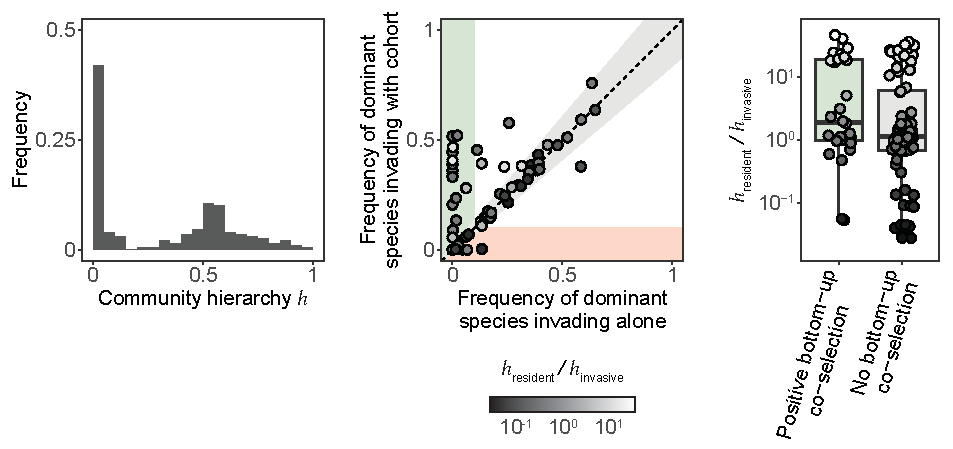
\includegraphics[scale=0.7,keepaspectratio]{figs/fig5.pdf}
\caption{\textbf{Community hierarchies determine coalescence outcomes.}
\textbf{a.} Blablabla...
\textbf{b.} Blablabla...
\textbf{b.} Blablabla... ($p=0.083$).}
\label{fig5}
\end{figure}

\clearpage

\section*{Supplementary Figures}

\renewcommand{\thefigure}{S\arabic{figure}}
\setcounter{figure}{0} 

\begin{figure}[!h]
\centering
\internallinenumbers
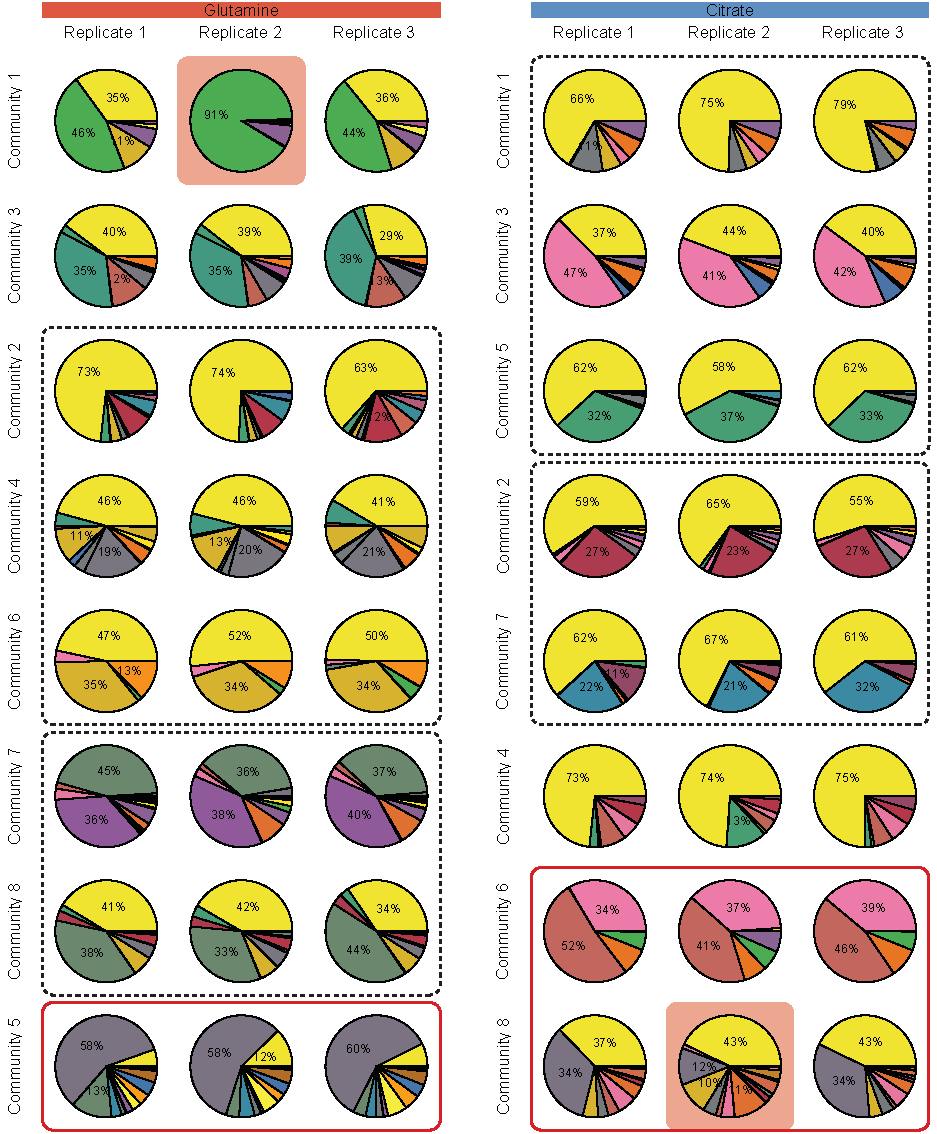
\includegraphics[scale=0.9,keepaspectratio]{figs/figS1.pdf}
\caption{\textbf{Community compositions after seven additional transfers without coalescence.}
Each color of the pie plots corresponds to a different exact sequence variant
(\methodsref{sequencing}).
Replicate 2 of community 1 from glutamine,
as well as replicate 2 of community 8 from citrate (highlighted) were removed based on their
dissimilarity to the other two replicates (details in code for data analysis, see
\nameref{datacode}).
Communities clustered in dashed boxes shared the same dominant species as revealed by
sequencing data.
For communities enclosed in red boxes, sequencing data showed that the species isolated by plating
was not detectable in the community after seven additional transfers (i.e. the dominant was
incorrectly identified) and were therefore excluded from downstream analyses.}
\label{figS1}
\end{figure}

\clearpage

\begin{figure}[!h]
\centering
\internallinenumbers
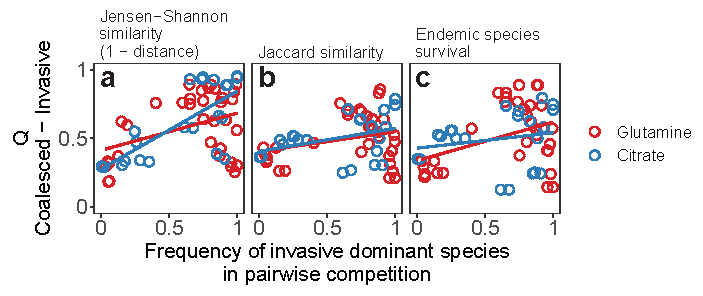
\includegraphics[scale=0.9,keepaspectratio]{figs/figS2.pdf}
\caption{\textbf{Alternative metrics of community distance.}
Quantifying coalescence outcomes using different metrics of community similarity
(\methodsref{metrics}) gives similar results to those shown in \figref[a]{fig2}.
Metrics that account for the relative species abundances (Bray-Curtis or Jensen-Shannon similarities)
yield higher correlations than less quantitative metrics that only
account for species presence/absence (Jaccard similarity or the fraction of endemic
invasive species persisting in the coalesced community).
\textbf{a.} Relative Jensen-Shannon similarity 
($R^2=0.15$, $p<0.05$ for glutamine and $R^2=0.53$, $p<5\times10^{-4}$ for citrate)
\textbf{b.} Relative Jaccard similarity
($R^2=0.08$, $p>0.05$ for glutamine and $R^2=0.13$, $p>0.05$ for citrate)
\textbf{c.} Relative survival of invasive endemic species after coalescence
($R^2=0.16$, $p<0.05$ for glutamine and $R^2=0.04$, $p>0.05$ for citrate).}
\label{figS2}
\end{figure}

\clearpage

\begin{figure}[!h]
\centering
\internallinenumbers
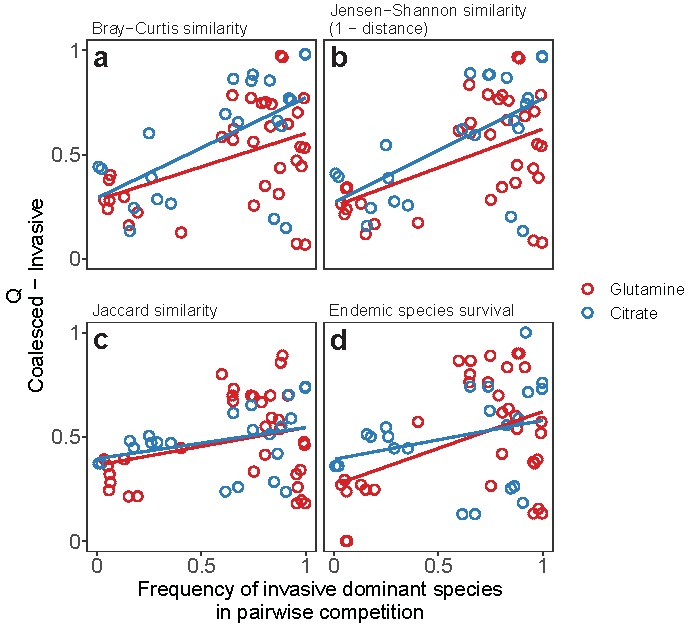
\includegraphics[scale=0.9,keepaspectratio]{figs/figS3.pdf}
\caption{\textbf{Dominant species have limited effects on coalescence outcomes quantification.}
We repeated the analyses shown in \figref[a]{fig2} and \figref{figS2}, but this time we removed the
dominants from the compositional data prior to quantifying community distances.
The trends observed before are maintained.
\textbf{a.} Relative Bray-Curtis similarity
($R^2=0.20$, $p<0.01$ for glutamine and $R^2=0.34$, $p<0.005$ for citrate)
\textbf{b.} Relative Jensen-Shannon similarity 
($R^2=0.24$, $p<0.005$ for glutamine and $R^2=0.36$, $p<0.005$ for citrate)
\textbf{c.} Relative Jaccard similarity
($R^2=0.09$, $p>0.05$ for glutamine and $R^2=0.11$, $p>0.05$ for citrate)
\textbf{d.} Relative survival of invasive endemic species after coalescence
($R^2=0.18$, $p<0.05$ for glutamine and $R^2=0.08$, $p>0.05$ for citrate).}
\label{figS3}
\end{figure}

\clearpage

\end{document}




















